\documentclass[12pt]{article}

\RequirePackage{iftex}
\ifPDFTeX
\usepackage[utf8]{inputenc}
\usepackage[T1]{fontenc}
\usepackage{newunicodechar}
\newunicodechar{Δ}{$\Delta$}
\fi

\usepackage{microtype}
\emergencystretch=2em

\usepackage{misqstyle}

\usepackage[
  style=apa,
  backend=biber,
  uniquelist=false,
  uniquename=false
]{biblatex}
\addbibresource{references.bib}

% Extra packages used in this paper
\usepackage{amsmath,amssymb}
\usepackage{booktabs}
\usepackage{graphicx}
\usepackage{array}
\usepackage{multirow}
\usepackage{xcolor}
\usepackage{hyperref}
\hypersetup{colorlinks=true, linkcolor=black, citecolor=black, urlcolor=black}

\title{Tracking Evolving Exploit Discourse in Hacker Communities: A Diachronic Exploit Text Graph Framework for Proactive Cyber Threat Intelligence}

\author{%
  Benjamin M.\ Ampel%
    \thanks{Corresponding author. University of Arizona, Tucson, AZ 85721. Email: bampel@arizona.edu}
  \and
  Sagar Samtani%
    \thanks{Kelley School of Business, Indiana University, Bloomington, IN 47405.}%
}
\date{}

\begin{document}
\frenchspacing
\pagenumbering{arabic}

% ── Title Page ─────────────────────────────────────────────────────────────────
\begin{titlepage}
\thispagestyle{plain}
\noindent
\begin{flushleft}

\includegraphics[height=1.5cm]{images/MISQ_logo.png}
\end{flushleft}
\vspace*{0.5cm}

\centering
\singlespacing
\makeatletter
{\fontsize{20}{24}\selectfont\bfseries\titlefont\@title\par}
\makeatother

\vspace{0.5cm}

\begin{abstract}
\setstretch{2.0}
\justifying
\itshape
\abstractfont
Cybersecurity threats emerge and evolve in hacker communities long before they are formally catalogued in vulnerability databases, yet existing threat-intelligence systems process static snapshots of hacker discourse, missing the temporal semantic drift that signals emerging attack patterns. We present the \textbf{Exploit Text Graph (ETG)}---a cumulative temporal co-occurrence graph of exploit vocabulary---and the \textbf{Diachronic Graph Transformer (DGT)}, a masked graph-attention model that embeds ETG nodes across successive temporal spells and predicts which terms will undergo the greatest semantic shift in the next observation window. Applied to HackerSignal, a 1,783,276-post multi-source corpus spanning 12 temporal spells from January 2016 through April 2026, DGT achieves a heldout mean absolute error of 0.0816 on next-spell shift prediction and significantly outperforms all 36 of 36 tested external benchmark models---including GloVe, PPMI, SGNS, and five dynamic graph neural network baselines---at a false-discovery-rate-corrected $q < 0.05$. Ablation experiments validate four design principles: cumulative graph encoding, adjacency-constrained self-attention with Laplacian positional encodings, a recency-weighted temporal context loss, and multi-source corpus construction. A six-term case study traces semantically pivotal cybersecurity events---from the Mirai botnet and WannaCry through the emergence of Ransomware-as-a-Service and LLM jailbreaking---demonstrating that DGT detects vocabulary realignment in real time and produces an actionable forward-looking watchlist of predicted next-spell shifts. Theoretical contributions, design principles, and practitioner implications for proactive cyber threat intelligence are discussed.
\end{abstract}

\vspace{0.75cm}

\begin{flushleft}
\justifying
\textbf{Keywords:} cyber threat intelligence, design science research, diachronic graph transformer, exploit text graph, hacker forum analytics, temporal semantic shift
\end{flushleft}

\vfill
\end{titlepage}
\stepcounter{page}

% ── Page 2: Title + Introduction ───────────────────────────────────────────────
\newpage
\singlespacing
\centering
\makeatletter
{\fontsize{20}{24}\selectfont\bfseries\titlefont\@title\par}
\makeatother
\setstretch{2}
\normalsize

\vspace{0.5cm}

% ═══════════════════════════════════════════════════════════════════════════════
\section{Introduction}
% ═══════════════════════════════════════════════════════════════════════════════
\setstretch{2}\normalsize\justifying\bodyfont

The cybersecurity threat landscape is defined by an asymmetric detection lag: adversaries develop, refine, and share novel attack techniques in hacker forums long before those techniques enter the formal record of known vulnerabilities. By the time a vulnerability receives a Common Vulnerabilities and Exposures (CVE) identifier and appears in catalogues such as the CISA Known Exploited Vulnerabilities (KEV) list, security teams face a compressed remediation window---often measured in days \parencite{jacobs2021, cisa2024}. Our analysis of 1,783,276 hacker-forum posts collected between January 2016 and April 2026 reveals that 271,275 distinct CVE identifiers were mentioned in hacker discourse, reflecting a vast pool of vulnerability intelligence that circulates in underground communities well before, during, and after formal classification. Bridging this information gap is a central challenge for proactive cyber threat intelligence (CTI).

Hacker communities are early-warning systems for emerging threats. Prior research in IS cybersecurity analytics has demonstrated that dark-web forums, hacker boards, and underground marketplaces contain signals predictive of real-world exploit activity \parencite{samtani2017, samtani2022, ebrahimi2022, nunes2016}. These communities develop, contest, and evolve a shared technical vocabulary---a lexicon in which terms not only denote artifacts (tools, vulnerabilities, techniques) but also encode the community's collective understanding of how those artifacts relate to one another. The vocabulary itself is dynamic: the word \textit{jailbreak} referred exclusively to iOS firmware bypass through 2022 before migrating, almost entirely, to large-language-model (LLM) safety-filter circumvention following the public release of ChatGPT. The word \textit{stealer} shifted from a generic adjective to a recognised product category (e.g., RedLine Stealer, Raccoon Stealer) with versioned releases and subscription pricing. Tracking these \textit{semantic shifts}---changes in how terms are used relative to their co-occurrence neighbours---offers a mechanism for detecting emerging attack paradigms before they crystallise into named CVEs.

Despite this potential, existing IS cybersecurity analytics systems treat hacker discourse as a static or bag-of-words phenomenon. Text-mining methods \parencite{samtani2017, tavabi2018}, deep transfer learning \parencite{samtani2022}, and cross-lingual models \parencite{ebrahimi2022} extract threat signals from individual snapshots or aggregate corpora, but none model the continuous temporal drift of exploit vocabulary as a predictive signal. Classical diachronic semantic models \parencite{hamilton2016, kim2014} capture word-level drift but discard the relational co-occurrence structure that encodes how exploit techniques combine---a structure central to understanding attack chains. Dynamic graph neural networks \parencite{sankar2020, rossi2020} model temporal graph evolution but are not designed for the shift-prediction task or for the cumulative nature of exploit knowledge. The result is a methodological gap: no prior IS artifact simultaneously (1) represents exploit discourse as a relational graph, (2) learns diachronic embeddings across sequential graph snapshots, and (3) forecasts next-period semantic shift to support proactive CTI.

We address this gap through a Design Science Research \parencite{hevner2004, peffers2007} programme that produces two interlocking IS artifacts. The \textbf{Exploit Text Graph (ETG)} is a cumulative directed weighted graph in which nodes represent stemmed exploit terms and edges represent co-occurrence within a four-token sliding window across all posts up to and including each temporal spell. The ETG grows monotonically---capturing the accumulation of community knowledge---and is constructed at 12 spell boundaries spanning a decade of hacker discourse. The \textbf{Diachronic Graph Transformer (DGT)} is an adjacency-constrained graph-attention encoder trained on the sequence of ETG snapshots to produce per-term embeddings whose cosine distance between consecutive spells quantifies semantic shift. Next-spell shift forecasting is performed post-hoc---after training---by applying EMA extrapolation to the per-spell embedding trajectories, enabling the construction of a forward-looking watchlist of terms expected to undergo the greatest semantic realignment.

This paper makes three primary contributions to IS research and practice. First, we contribute two novel IS artifacts---the ETG and DGT---accompanied by four empirically validated design principles. Second, we contribute a rigorous 38-model benchmark evaluation spanning non-neural diachronic baselines, static and dynamic graph embeddings, and modern graph transformers, with paired significance testing and false-discovery-rate correction. Third, we contribute a six-term case study grounded in publicly verifiable cybersecurity events, demonstrating that DGT correctly identifies semantic pivots associated with the Mirai botnet, WannaCry/EternalBlue, Ransomware-as-a-Service emergence, info-stealer marketplaces, Ivanti zero-days, and LLM jailbreaking---each a shift that a practitioner would recognise as a meaningful change in the threat landscape.

The remainder of this paper is organised as follows. Section 2 reviews related work across four theoretical streams. Section 3 describes the Design Science Research approach. Section 4 presents the artifact design. Section 5 reports the benchmark evaluation. Section 6 presents the case study. Section 7 discusses theoretical contributions, practical implications, and limitations. Section 8 concludes.

% ═══════════════════════════════════════════════════════════════════════════════
\section{Theoretical Background and Related Work}
% ═══════════════════════════════════════════════════════════════════════════════
\bodyfont

\subsection{IS Cybersecurity Analytics and Hacker Community Intelligence}

Hacker communities---including dark-web forums, surface-web hacker boards, and underground marketplaces---have become a primary data source for proactive cybersecurity analytics in the IS literature. Foundational work by \textcite{samtani2017} introduced a hacker asset framework that identifies emerging tools, exploits, and key actors in hacker forums, demonstrating that community-level text analytics can surface intelligence unavailable from traditional vulnerability feeds. Subsequent work extended this framework to link dark-web exploit postings to known CVEs using semantic embedding techniques, showing that deep representations of hacker posts can predict exploitation activity \parencite{samtani2022}. Cross-lingual extensions \parencite{ebrahimi2022} addressed the multilingual character of global hacker communities, applying zero-shot and adversarial learning methods to non-English forums, while vulnerability prioritisation research \parencite{ullman2024} demonstrated that multi-view learning over vulnerability metadata improves CVSS scoring and KEV classification.

A parallel literature focuses on SCADA and IoT vulnerability intelligence, extracting structured threat indicators from unstructured hacker posts \parencite{samtani2020}, and on the epidemiology of exploit diffusion through underground networks \parencite{nunes2016, tavabi2018}. Collectively, this body of work establishes that hacker communities are rich, timely, and idiosyncratic sources of threat intelligence---but it also reveals a shared limitation: all existing IS cybersecurity analytics methods process hacker discourse at a single point in time or aggregate across time, treating the corpus as a static collection. None model how the \textit{meaning} of exploit terms evolves continuously, nor do they forecast which terms are approaching a semantic transition. Our work directly addresses this gap.

\subsection{Diachronic Semantic Models}

Diachronic (time-varying) semantic models seek to track how the meaning of words changes across corpora collected at different time periods. The foundational approach of \textcite{hamilton2016} trains Word2Vec embeddings \parencite{mikolov2013} on successive temporal corpora and aligns them using Procrustes rotation, yielding cosine distances that measure per-word semantic change. \textcite{kim2014} extended this approach with temporal neural language models that explicitly condition word representations on time. \textcite{kulkarni2015} proposed statistical tests for detecting significant linguistic change in large corpora. More recently, \textcite{rottger2021} demonstrated that fine-tuning BERT \parencite{devlin2019} on time-stamped data improves temporal adaptation on downstream tasks, though at the cost of retraining for each new time period.

These methods share a fundamental limitation for the CTI application: they operate at the word level and discard the relational structure of co-occurrence. In hacker discourse, meaning is conveyed not only by individual terms but by the combinations of terms that co-occur---\textit{ransomware} and \textit{affiliate} co-occurring with \textit{panel} signals a different context than \textit{ransomware} co-occurring with \textit{decryption}. A graph representation captures this combinatorial semantics explicitly, enabling the model to detect when a term's neighbourhood changes---which is, precisely, what semantic shift means in a community of practice. Furthermore, diachronic word embedding methods are designed to measure shift, not to \textit{predict} it. Our DGT produces per-spell embeddings from which next-spell cosine shift is forecast post-hoc via EMA extrapolation, enabling proactive rather than retrospective analysis.

\subsection{Graph Neural Networks and Dynamic Graph Learning}

Graph neural networks (GNNs) generalise deep learning to graph-structured data by propagating information across node neighbourhoods \parencite{kipf2017, velickovic2018, hamilton2017graphsage}. Graph embedding methods---DeepWalk \parencite{perozzi2014}, Node2Vec \parencite{grover2016}, LINE \parencite{tang2015line}---learn static node representations by factorising adjacency or applying random walks, providing strong baselines for co-occurrence graph representation. For temporal graphs, dynamic graph neural networks model evolving node states: DySAT \parencite{sankar2020} applies self-attention across structural and temporal dimensions; EvolveGCN \parencite{pareja2020} uses recurrent units to evolve GCN weight matrices; TGN \parencite{rossi2020} combines memory modules with graph attention; and JODIE \parencite{kumar2019} projects user and item trajectories through time. These models have been applied to link prediction and node classification on interaction graphs, but not to the diachronic co-occurrence graph setting or the shift-prediction objective.

Graph Transformers adapt the self-attention mechanism \parencite{vaswani2017} to graph inputs. GraphGPS \parencite{rampasek2022} integrates local MPNN layers with global attention and Laplacian positional encodings \parencite{kreuzer2021}. TokenGT \parencite{kim2022tokengt} treats graphs as sequences of node and edge tokens, enabling full quadratic attention. These architectures excel on molecular property prediction and graph classification benchmarks, but have not been applied to temporal co-occurrence graphs in the NLP or security domain. Our DGT adapts the graph transformer paradigm specifically for diachronic exploit graph embedding by introducing adjacency-constrained within-spell attention---restricting self-attention to ETG co-occurrence neighbours so that each node's representation encodes relational graph semantics rather than global term proximity---combined with a recency-weighted temporal context loss that enforces temporally ordered embedding trajectories. Post-hoc EMA extrapolation over the resulting per-spell embeddings then yields a shift forecast absent from all prior graph transformer formulations.

\subsection{The ETG and DGT Paradigm: Filling the Gap}

\begin{misqtable}{6}{Comparison of Related Work on Key Dimensions}%
{Note: $\checkmark$ = supported; $\times$ = not supported; $\sim$ = partially supported. \textit{IS Domain} refers to hacker-community or cybersecurity analytics; \textit{Graph Structure} to relational co-occurrence representation; \textit{Temporal} to sequential spell modelling; \textit{Shift Prediction} to forecasting next-period semantic change.}%
{l|p{2.6cm}|c|c|c|c}
\textbf{Approach} & \textbf{Representative Works} & \textbf{IS Domain} & \textbf{Graph} & \textbf{Temporal} & \textbf{Shift Pred.} \\
\hline
IS CTI Analytics    & \citeauthor{samtani2017} (\citeyear{samtani2017, samtani2022}) & $\checkmark$ & $\times$ & $\times$ & $\times$ \\
\hline
Diachronic Semantics & \citeauthor{hamilton2016} (\citeyear{hamilton2016}); \citeauthor{kim2014} (\citeyear{kim2014}) & $\times$ & $\times$ & $\checkmark$ & $\times$ \\
\hline
Dynamic GNNs        & \citeauthor{rossi2020} (\citeyear{rossi2020}); \citeauthor{sankar2020} (\citeyear{sankar2020}) & $\times$ & $\checkmark$ & $\checkmark$ & $\times$ \\
\hline
Graph Transformers  & \citeauthor{rampasek2022} (\citeyear{rampasek2022}); \citeauthor{kim2022tokengt} (\citeyear{kim2022tokengt}) & $\times$ & $\checkmark$ & $\times$ & $\times$ \\
\hline
\textbf{ETG + DGT (ours)} & This paper & $\checkmark$ & $\checkmark$ & $\checkmark$ & $\checkmark$ \\
\hline
\end{misqtable}

As shown in Table 1, no prior work occupies all four dimensions simultaneously. The ETG fills the relational IS-domain gap by constructing a cumulative graph of exploit co-occurrences grounded in hacker forum data. The DGT fills the temporal shift-prediction gap by applying adjacency-constrained graph-attention within each ETG snapshot, training with a recency-weighted temporal context loss to enforce diachronically ordered embedding trajectories, and forecasting next-period cosine drift post-hoc via EMA extrapolation. Together, they instantiate four design principles derived from this gap analysis:

\begin{itemize}
  \item \textbf{DP1 --- Cumulative Encoding:} Exploit knowledge accumulates; each spell's graph should encode all prior co-occurrence evidence, not only the current period.
  \item \textbf{DP2 --- Adjacency-Constrained Self-Attention:} Attention between nodes is restricted to observed ETG co-occurrence neighbours, encoding relational exploit structure. Nodes additionally carry Laplacian spectral positional encodings that ground representations in graph topology. Temporal isolation is enforced architecturally through per-spell independent encoding.
  \item \textbf{DP3 --- Recency-Weighted Temporal Context Loss:} The training objective includes a novel EMA-based regulariser encouraging temporal continuity in embedding space, pulling current-spell embeddings toward a smooth exponential average of past spell embeddings so that diachronic trajectories remain ordered and smooth across spells.
  \item \textbf{DP4 --- Multi-Source Corpus:} Threat intelligence requires breadth; the corpus must combine hacker communities, vulnerability references, advisories, exploit archives, and related sources.
\end{itemize}

% ═══════════════════════════════════════════════════════════════════════════════
\section{Design Science Research Approach}
% ═══════════════════════════════════════════════════════════════════════════════
\bodyfont

\subsection{DSR Methodology}

We adopt the Design Science Research methodology of \textcite{hevner2004}, which frames IS research as the creation and evaluation of purposeful artifacts that address organisational problems. The three DSR cycles---relevance, design, and rigor---structure our work. The relevance cycle grounds the research in the practitioner need for proactive CTI. The design cycle encompasses the construction and instantiation of the ETG and DGT artifacts. The rigor cycle connects the artifacts to the prior knowledge base in diachronic semantics, graph learning, and IS cybersecurity analytics. We additionally apply the six-step DSRM process of \textcite{peffers2007}: problem identification, objectives of a solution, design and development, demonstration, evaluation, and communication \parencite{gregor2013}.

\subsection{Problem Relevance}

The practitioner problem is well-documented: CTI analysts at security operations centres, CISOs at enterprise organisations, and analysts at Information Sharing and Analysis Centres (ISACs) require timely intelligence about emerging threats. Existing tools---SIEM platforms, signature-based intrusion detection, static vulnerability feeds---are reactive; they alert after an attack technique is known and catalogued. Hacker forums contain this information earlier, but no IS artifact operationalises the temporal dimension of that intelligence. The problem is an IS problem---not a purely technical one---because it involves the design of an artifact for a knowledge-work context (CTI analysis), requires organisational data (multi-source hacker corpora), and has implications for managerial decision-making (vulnerability prioritisation, resource allocation for patching).

\subsection{Design Objectives}

Three design objectives flow directly from the problem and the gap analysis in Section 2.4. First, the artifact must \textit{represent exploit relationships} as a graph, capturing how terms co-occur and combine. Second, it must \textit{model temporal drift} across successive observation periods, learning embeddings that encode semantic evolution. Third, it must \textit{generate actionable predictions}---a ranked watchlist of terms predicted to shift meaning in the next period---that a CTI analyst can operationalise without additional modelling expertise. These objectives map directly to the ETG, the DGT encoder, and the watchlist generation procedure, respectively.

\subsection{Evaluation Strategy}

Following \textcite{hevner2004}'s taxonomy of evaluation modes, we employ two complementary approaches. First, a \textit{technical evaluation} benchmarks DGT against 38 models across four experiment tiers---non-neural diachronic baselines, graph embedding and dynamic GNN baselines, modern graph transformers, and DGT component ablations---with paired significance testing and Benjamini--Hochberg false discovery rate correction \parencite{benjamini1995}. This evaluation addresses the question of whether DGT advances the state of the art on the shift-prediction task. Second, a \textit{naturalistic evaluation} presents a six-term case study anchored to publicly verifiable real-world cybersecurity events, demonstrating the artifact's practical utility without requiring a controlled laboratory study. A formal user study with CTI practitioners is identified as priority future work.

% ═══════════════════════════════════════════════════════════════════════════════
\section{Artifact Design}
% ═══════════════════════════════════════════════════════════════════════════════
\bodyfont

\subsection{HackerSignal Corpus}

\subsubsection{The Full HackerSignal Dataset}

The ETG analysis draws on HackerSignal \parencite{ampel2026hackersignal}, a large-scale multi-source benchmark corpus linking hacker community discourse to the CVE vulnerability lifecycle. The full HackerSignal release comprises \textbf{7,447,646 exact-deduplicated documents} from \textbf{64 public forum and source identifiers} spanning \textbf{eight source layers} and a \textbf{36-year window} (1991--2026):

\begin{enumerate}
  \item \textbf{Hacker Community (6,966,014 docs; 56 forums):} Organic security discourse from darkweb marketplaces, security discussion boards, and multilingual hacker communities. Major forums include \texttt{gayanku\_darkweb} (3.11M rows, 2011--17), \texttt{antichat} (1.82M, 2002--26), \texttt{evolution\_darkweb} (471K, 2014--15), \texttt{antionline} (463K, 2001--26), \texttt{persiantools} (280K), \texttt{wwhclub} (161K), and \texttt{hackforums} (151K, 2009--15), alongside 48 additional forums.
  \item \textbf{Vulnerability Reference (340,536 docs):} National Vulnerability Database (NVD) CVE descriptions (2002--26), each with a CVE identifier; the retrieval corpus for HackerSignal's benchmark tasks.
  \item \textbf{Exploit Archive (46,653 docs):} ExploitDB, 0day.today, PacketStorm, ZeroScience, and Vulnerability-Lab proof-of-concept exploit descriptions (1991--2026).
  \item \textbf{Exploit Q\&A Reference (46,505 docs):} Structured exploit question-and-answer references (circa 2000).
  \item \textbf{Advisory Reference (28,684 docs):} GitHub Advisory, CISA advisories, and CERT notices (2017--2026).
  \item \textbf{Bug-Bounty Disclosure (9,453 docs):} HackerOne and related bug-bounty platform reports (2013--2024).
  \item \textbf{Fix-Commit Reference (8,293 docs):} CVEfixes security-relevant fix commit messages (1999--2022).
  \item \textbf{Exploitation Reference (1,508 docs):} CISA Known Exploited Vulnerabilities (KEV) catalog entries (2021--2026).
\end{enumerate}

Documents are unified through a shared CVE identifier namespace and a common JSONL record format carrying source provenance, ISO~8601 timestamps, and pseudonymized author hashes. Across all 7.45M documents, 4.8\% carry explicit CVE references, 23.5\% contain at least one CTI keyword, and estimated near-duplicates account for 8.2\% (addressed through SHA-256 exact deduplication and MinHash-LSH near-deduplication during corpus construction). The corpus spans multilingual content---including Russian, Turkish, Persian, Arabic, and Chinese in DeepDarkCTI and darknet sources---though English-language posts constitute the substantial majority.

\subsubsection{ETG Corpus: Subsetting HackerSignal to the Analysis Window}

The ETG analysis requires a \textit{temporally coherent} corpus aligned with the modern era of systematic CVE tracking and structured exploit discourse. We apply a single temporal filter: \textbf{January 1, 2016 onward}. The 2016 boundary is motivated by three converging factors. First, the CISA KEV catalog, the NVD's modern structured CVE format, and the major hacker community platforms that dominate our analysis all reach maturity and consistent coverage after 2016. Second, the pre-2016 period is dominated by a small number of historical forum archives (Gayanku 2011--17, Evolution 2014--15) whose temporal coverage is asymmetric with respect to the other source layers. Third, the ETG's design is oriented toward the \textit{modern} exploit discourse era---the decade in which IoT weaponisation, ransomware-as-a-service, nation-state zero-day exploitation, and LLM safety bypass all emerged as dominant threat paradigms.

Applying the 2016+ filter to HackerSignal yields the \textbf{ETG corpus of 1,783,276 documents} across \textbf{seven active source layers} (Table 2). The Exploit Q\&A Reference layer (46,505 documents, circa 2000) falls entirely outside the analysis window and is excluded. All other layers are retained but reduced in size relative to the full HackerSignal release; the largest reduction occurs in the Hacker Community layer (6,966,014 $\rightarrow$ 1,455,413), primarily because Gayanku (2011--17), Evolution (2014--15), HackForums (2009--15), and other historical archives largely predate our cutoff.

\begin{misqtable}{5}{ETG Corpus Source Layer Statistics (HackerSignal Subset, 2016--2026)}%
{Note: The ETG corpus is derived from HackerSignal \parencite{ampel2026hackersignal} by applying a January 2016 temporal cutoff. The full HackerSignal release contains 7,447,646 documents across 8 source layers (1991--2026); the Exploit Q\&A Reference layer (46,505 docs, circa 2000) is excluded by the cutoff. Percentages may not sum to 100 due to rounding.}%
{l|r|r|r|l}
\textbf{Source Layer} & \textbf{ETG Corpus} & \textbf{\%} & \textbf{Full HackerSignal} & \textbf{Primary Content} \\
\hline
Hacker Community         & 1,455,413 & 81.6 & 6,966,014 & Forum posts, tool releases, community discourse \\
\hline
Vulnerability Reference  & 270,515   & 15.2 & 340,536   & NVD CVE descriptions \\
\hline
Advisory Reference       & 28,684    & 1.6  & 28,684    & GitHub Advisory, CISA advisories \\
\hline
Exploit Archive          & 11,652    & 0.65 & 46,653    & PoC exploit descriptions (ExploitDB, etc.) \\
\hline
Bug Bounty Disclosure    & 8,338     & 0.47 & 9,453     & HackerOne reports \\
\hline
Fix Commit Reference     & 7,166     & 0.40 & 8,293     & Security fix commit messages \\
\hline
Exploitation Reference   & 1,508     & 0.08 & 1,508     & CISA KEV entries \\
\hline
\textbf{ETG Total}       & \textbf{1,783,276} & \textbf{100.0} & \textbf{7,447,646} & \\
\hline
\end{misqtable}

This multi-source design instantiates DP4: no single source captures the full semantic spectrum of exploit vocabulary in use. Hacker communities supply the raw, early-stage discourse; vulnerability references provide formal CVE-grounded vocabulary; advisory and exploit archive layers contribute the technical detail that distinguishes attack-oriented usage from general security discussion; and the KEV exploitation layer grounds the corpus in confirmed, weaponised vulnerabilities.

Each post is preprocessed through a standard pipeline: Unicode normalisation, lowercasing, tokenisation, Porter stemming, stopword removal, and CVE-ID extraction (matching the pattern \texttt{CVE-YYYY-NNNN}). A four-token sliding window is applied to each post's token sequence to enumerate ordered co-occurrence pairs: for each token $u$ at position $i$, edges $(u, v)$ are created for each $v$ in positions $i{+}1$ through $i{+}4$. Co-occurrence counts accumulate into the ETG for each spell. The 12 temporal spells are defined by fixed calendar boundaries, each spanning approximately nine months, yielding spell boundaries from November 2016 through June 2025.

\subsection{Exploit Text Graph Construction}

\subsubsection{Formal Definition}

The Exploit Text Graph at spell $t$ is a directed weighted graph $\mathcal{G}_t = (\mathcal{V}, \mathcal{E}_t, \mathbf{W}_t)$, where $\mathcal{V}$ is the vocabulary of stemmed exploit terms, $\mathcal{E}_t \subseteq \mathcal{V} \times \mathcal{V}$ is the edge set, and $\mathbf{W}_t : \mathcal{E}_t \rightarrow \mathbb{R}_{>0}$ assigns co-occurrence weights. An edge $(u, v) \in \mathcal{E}_t$ exists if $u$ precedes $v$ within a four-token sliding window in at least one post up to and including spell $t$, capturing sequential proximity; its weight is the cumulative count of such co-occurrences. Only edges with weight $\geq 10$ (minimum co-occurrence threshold) are retained per spell, and the top 300,000 edges by weight are kept to bound memory.

\subsubsection{Cumulative Design (DP1)}

Crucially, $\mathcal{G}_t$ is \textit{cumulative}: it incorporates all posts from the corpus inception through the end of spell $t$. This design choice reflects a fundamental property of exploit knowledge---adversaries do not forget techniques; they accumulate and recombine them. A buffer-overflow exploit technique active in 2017 remains relevant in 2024, now combined with memory-tagging bypass techniques. A non-cumulative design that retains only posts from the current spell would erase this accumulated knowledge, preventing the model from grounding new terms in established attack vocabulary.

\subsubsection{Node Features}

Each node $v \in \mathcal{V}$ at spell $t$ is associated with a 9-dimensional base feature vector, with all frequency counts log-transformed via $\log(1+x)$ to compress the heavy-tailed distribution: (1) log term frequency $\log(1+f_t(v))$, (2) log document frequency $\log(1+d_t(v))$, (3) log in-degree $\log(1+\text{deg}^-(v))$, (4) log out-degree $\log(1+\text{deg}^+(v))$, (5) log weighted in-degree $\log(1+\sum_{u:(u,v)\in\mathcal{E}_t} W_t(u,v))$, (6) log weighted out-degree $\log(1+\sum_{v:(v,w)\in\mathcal{E}_t} W_t(v,w))$, (7) normalised word length $|v|/32$, (8) a binary flag for digit-containing terms (e.g., CVE IDs, version numbers), and (9) a binary flag for terms containing non-alphanumeric characters (e.g., hyphenated tokens). These nine scalar features capture distributional prominence, graph centrality, and basic lexical morphology. Graph-structural position is encoded separately via Laplacian positional encodings (Section~4.3.2).

\subsubsection{Growth Statistics}

Table 3 reports ETG statistics at four representative spells. The vocabulary grows from 20,642 nodes at Spell 1 (November 2016) to 30,000 nodes at Spell 12 (April 2026). Edges are capped at 300,000 per spell---retaining the top-weighted co-occurrence pairs---to bound computational cost. The cumulative co-occurrence weight grows from 11.6 million at Spell 1 to 55.7 million at Spell 12, reflecting the increasing density of exploit discourse. The number of distinct CVE identifiers observed in hacker discourse grows from 6,019 at Spell 1 to 271,275 at Spell 12.

\begin{misqtable}{6}{Exploit Text Graph Growth Across Representative Spells}%
{Note: Edges capped at 300,000 per spell (top-weighted pairs retained). Full 12-spell statistics in Appendix A.}%
{l|l|r|r|r|r}
\textbf{Spell} & \textbf{Date Range} & \textbf{Posts} & \textbf{Nodes} & \textbf{Edges} & \textbf{CVEs Obs.} \\
\hline
S01 & Jan 2016 -- Nov 2016 & 330,404   & 20,642 & 280,344 & 6,019   \\
\hline
S04 & Jul 2018 -- Jun 2019 & 774,023   & 24,526 & 300,000 & 50,748  \\
\hline
S08 & Jan 2022 -- Nov 2022 & 1,100,924 & 27,994 & 300,000 & 126,118 \\
\hline
S12 & Jun 2025 -- Apr 2026 & 1,783,276 & 30,000 & 300,000 & 271,275 \\
\hline
\end{misqtable}

Figure 1 shows the growth of the ETG vocabulary (nodes) and edge weight (co-occurrence mass) across all 12 spells.

\begin{misqfigure}{Figure 1. Exploit Text Graph growth across 12 temporal spells (2016--2026). Left axis: vocabulary size (word nodes). Right axis: total co-occurrence edge weight. The steady accumulation of both nodes and edge weight reflects the expanding scope of hacker-forum exploit discourse over the decade.}
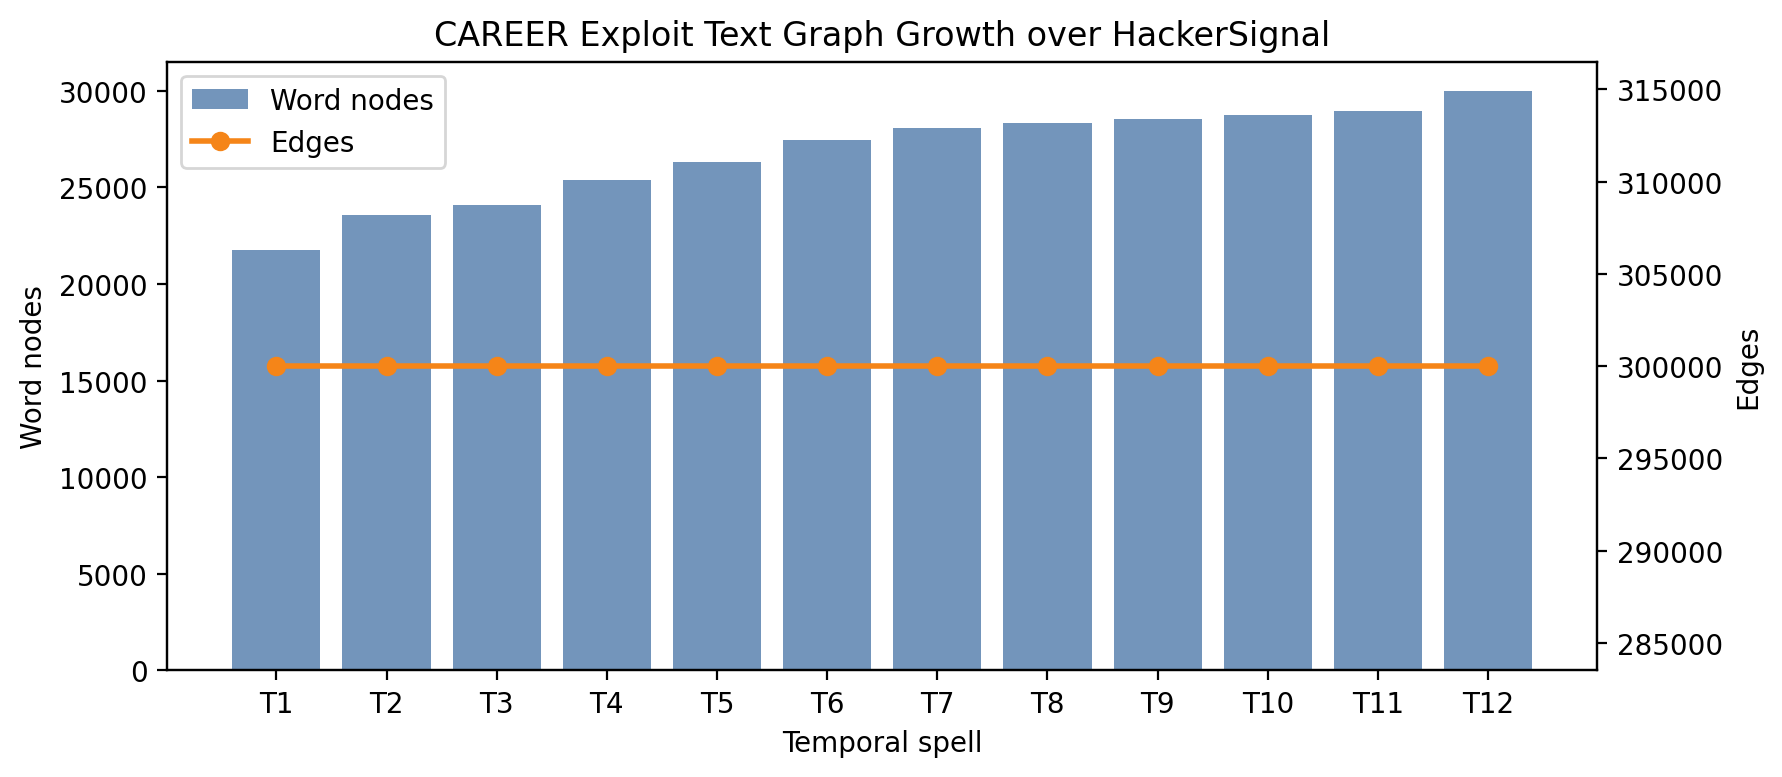
\includegraphics[width=0.92\textwidth]{images/career_etg_growth.png}
\end{misqfigure}

\subsection{Diachronic Graph Transformer Architecture}

\subsubsection{Input and Vocabulary}

The DGT operates on the top-$N = 6{,}000$ nodes ranked by raw term frequency in the final spell. Selecting vocabulary from the final spell ensures the embedding space is anchored to the most active terms in current discourse while remaining computationally tractable. The 9-dimensional base feature matrices $\mathbf{X}_t \in \mathbb{R}^{N \times 9}$ and Boolean adjacency matrices $\mathbf{A}_t \in \{0,1\}^{N \times N}$ for spells $t = 1, \ldots, T$ are constructed independently for each spell from the cumulative ETG snapshots and form the input to the DGT encoder.

\subsubsection{Adjacency-Constrained Attention and Structural Encodings (DP2)}

Following \textcite{kreuzer2021} and \textcite{rampasek2022}, we augment each node's feature vector with the $k = 16$ eigenvectors corresponding to the $k$ smallest non-trivial eigenvalues of the \textit{normalised} graph Laplacian:
\begin{equation}
  \mathbf{L}_t = \mathbf{I} - \mathbf{D}_t^{-1/2}\, \mathbf{A}_t\, \mathbf{D}_t^{-1/2}
\end{equation}
where $\mathbf{D}_t$ is the diagonal degree matrix. These Laplacian positional encodings (LapPE) give each node a structural fingerprint---its position in the graph's spectral geometry---that is sensitive to local co-occurrence topology without requiring global position labels. This is an established technique for injecting graph structure into otherwise position-agnostic transformers \parencite{kreuzer2021}. The augmented node representation is:
\begin{equation}
  \tilde{\mathbf{X}}_t = [\mathbf{X}_t \;\|\; \mathbf{\Phi}_t] \in \mathbb{R}^{N \times (9+k)}
\end{equation}
where $\mathbf{\Phi}_t \in \mathbb{R}^{N \times k}$ contains the $k$ eigenvectors, yielding a 25-dimensional input per node ($d_{\text{in}} = 9 + 16 = 25$).

\subsubsection{Adjacency-Masked Transformer Encoder}

\textit{What is standard practice.} The DGT's within-spell encoder is implemented as a two-layer PyTorch \texttt{TransformerEncoder} \parencite{vaswani2017} with GELU activation, $d = 128$ hidden dimensions, $h = 4$ attention heads, a $2d$-dimensional feedforward sublayer, and 0.2 dropout. The key structural adaptation---common to graph transformer approaches \parencite{rampasek2022}---is that the self-attention operation is constrained by the ETG adjacency matrix: tokens (nodes) that are not co-occurrence neighbours are blocked from attending to each other via a Boolean attention mask $\mathbf{M}_t \in \{0,1\}^{N \times N}$:
\begin{equation}
  \text{Attn}(\mathbf{Q},\mathbf{K},\mathbf{V})_{ij} = \frac{(\mathbf{Q}_i \cdot \mathbf{K}_j) / \sqrt{d_k} + m_{ij}}{\text{(softmax over } j\text{)}}
\end{equation}
where $m_{ij} = -\infty$ if $(i,j) \notin \mathcal{E}_t$ (non-neighbours are masked out) and $m_{ij} = 0$ otherwise. This constrains information flow to ETG co-occurrence structure without requiring explicit message-passing aggregation. Each spell's graph is encoded independently: the encoder is called once per spell $t$, producing per-spell node embeddings $\mathbf{E}_t \in \mathbb{R}^{N \times d}$ with parameters shared across all spells.

\textit{What is novel: temporal grounding and the residual bypass.} To inject temporal position, a \textit{learned spell-index embedding} $\mathbf{s}_t \in \mathbb{R}^d$ (implemented as a standard \texttt{nn.Embedding} table, one vector per spell) is added to each node's projected feature vector before encoding:
\begin{equation}
  \mathbf{h}_{v,t}^{(0)} = \mathbf{W}_{\text{in}}\,\tilde{\mathbf{x}}_{v,t} + \mathbf{s}_t
\end{equation}
This is the only mechanism by which the model learns that two calls with the same adjacency structure belong to different time periods. After encoding, a learnable scalar gating parameter $\alpha \in [0,1]$ (implemented as $\alpha = \sigma(\theta)$ with $\theta$ initialised to 0) forms a residual bypass between the raw projected input and the transformer output:
\begin{equation}
  \mathbf{z}_{v,t} = \alpha\,\mathbf{e}_{v,t}^{\text{enc}} + (1-\alpha)\,\mathbf{h}_{v,t}^{(0)}
\end{equation}
The final per-node embedding is produced by an MLP projection followed by L2 normalisation: $\mathbf{e}_{v,t} = \text{L2}(\mathbf{W}_2 \,\text{ReLU}(\mathbf{W}_1\, \mathbf{z}_{v,t}))$. The scalar $\alpha$ is jointly learned during training; it controls the trade-off between the structurally-enriched transformer representation and the raw (but temporally-grounded) input.

\textit{Temporal isolation and the no-masked-attention ablation.} Because each spell is processed by an independent forward pass, there is no cross-spell attention and therefore no risk of future-spell leakage within the encoder---temporal isolation is an architectural property, not the product of a causal mask. The within-spell adjacency mask $\mathbf{M}_t$ serves a different purpose: it prevents attention from propagating across non-co-occurrence pairs, ensuring that embeddings encode the ETG's relational structure rather than unconstrained global similarity. The ablation reported in Table~7---where replacing the adjacency-constrained attention with full within-spell attention ($\mathbf{M}_t = \mathbf{0}$, all nodes attend to all nodes) increases MAE by $\Delta = +0.054$---validates DP2's requirement that attention be structurally constrained. Temporal ordering across spells is enforced separately through the context loss described in Section~4.3.4 (DP3).

\subsubsection{Training Objective: Link Prediction and Temporal Context Loss (DP3)}

\textit{What is standard practice.} DGT is trained with a composite loss:
\begin{equation}
  \mathcal{L} = \mathcal{L}_{\text{link}} + \lambda\, \mathcal{L}_{\text{temporal}}, \quad \lambda = 0.1
\end{equation}
The primary term $\mathcal{L}_{\text{link}}$ is a standard binary cross-entropy link-prediction loss over sampled positive (observed co-occurrence) and negative (randomly drawn non-edge) node pairs, evaluated independently per spell:
\begin{equation}
  \mathcal{L}_{\text{link}} = -\!\sum_{t=1}^{T}\!\sum_{(u,v)}\!\Big[ y_{uv}\log\sigma(\mathbf{e}_{u,t}^{\top}\mathbf{e}_{v,t}) + (1-y_{uv})\log(1-\sigma(\mathbf{e}_{u,t}^{\top}\mathbf{e}_{v,t}))\Big]
\end{equation}
where $y_{uv}=1$ for observed ETG edges. Up to 65,536 positive pairs are sampled per spell per batch to bound GPU memory.

\textit{What is novel: recency-weighted temporal context loss.} The temporal term $\mathcal{L}_{\text{temporal}}$ is a novel regulariser that encourages temporal continuity in embedding space. For each spell $t > 1$, the current spell's embeddings are penalised for deviating from an \textit{exponentially-weighted moving average} (EMA) of all preceding spells' embeddings:
\begin{equation}
  \bar{\mathbf{E}}_{<t} = \sum_{s=1}^{t-1} w_s\, \mathbf{E}_s, \quad w_s \propto \exp\!\bigl(-0.5 \cdot (t-1-s)\bigr)
\end{equation}
\begin{equation}
  \mathcal{L}_{\text{temporal}} = \sum_{t=2}^{T} \bigl\| \mathbf{E}_t - \bar{\mathbf{E}}_{<t} \bigr\|_F^2
\end{equation}
The EMA weights assign the highest influence to the most recent past spell and exponential decay to earlier ones, so the model is pulled toward recent context rather than a flat historical average. Crucially, $\bar{\mathbf{E}}_{<t}$ is detached from the computation graph---only $\mathbf{E}_t$ contributes gradients---so the loss acts as a smoothness constraint on the current spell without backpropagating through all past embeddings. This design is novel: it imposes temporal ordering and smooth drift (DP3) on the embedding trajectory without requiring cross-spell attention or an explicit recurrence, while the per-spell independent encoding enforces temporal isolation (DP2) by architectural construction.

\textit{Optimisation.} Training uses AdamW (learning rate $10^{-3}$, weight decay $10^{-4}$) for 200 epochs with a linear warmup schedule (10\% of epochs) followed by cosine annealing to $10^{-5}$. Gradients are clipped to unit norm to stabilise training.

\subsubsection{Shift Prediction via Post-Hoc EMA Extrapolation (Novel)}

There is \textit{no learned shift-prediction head} in the DGT. Shift forecasting is performed post-hoc, after training, using the per-spell embeddings. For each term $v$, the sequence of observed cosine shifts across historical spell transitions is computed:
\begin{equation}
  c_{v,t} = 1 - \cos(\mathbf{e}_{v,t-1},\, \mathbf{e}_{v,t}), \quad t = 2, \ldots, T
\end{equation}
The predicted next-spell shift is then the recency-weighted EMA of historical shifts (decay $\gamma = 0.7$):
\begin{equation}
  \hat{y}_v = \sum_{t=2}^{T} w_t\, c_{v,t}, \quad w_t \propto \gamma^{T-t}, \quad \hat{y}_v \geq 0
\end{equation}
This approach uses no additional learned parameters beyond the encoder. Its novelty lies in the combination of structure-aware diachronic embeddings (which capture the \textit{direction} of semantic change, not just frequency) with a simple, interpretable extrapolation rule that is robust to outlier transitions. The design reflects a deliberate choice to separate representation learning (the encoder) from prediction (the EMA), keeping each component transparent and diagnosable.

\subsection{Shift Prediction and Watchlist Generation}

At inference, the trained encoder produces per-spell embeddings for all 6,000 tracked terms; consecutive-spell cosine shifts are computed, and the EMA extrapolation (Section~4.3.4) produces a predicted next-spell shift $\hat{y}_v$ for each term. Terms are ranked by $\hat{y}_v$ and the top-$n$ are filtered through a curated security annotation dictionary---a hand-crafted mapping from stemmed terms to plain-English security interpretations covering AI/LLM safety bypass, access control, memory safety, credential theft, network infrastructure, and vendor-specific vulnerability patterns. Terms that pass through the filter form the \textit{DGT Watchlist}: a ranked, annotated list of terms predicted to undergo the greatest semantic realignment in the forthcoming spell, delivered to CTI analysts as an actionable intelligence product.

% ═══════════════════════════════════════════════════════════════════════════════
\section{Evaluation}
% ═══════════════════════════════════════════════════════════════════════════════
\bodyfont

\subsection{Experimental Setup}

All models are evaluated on the same vocabulary of 6,000 terms and the same heldout target: the observed cosine shift at Spell 12 (the most recent spell, held out from training). Primary evaluation metrics are the mean absolute error (MAE) and root mean squared error (RMSE) of next-spell shift prediction, supplemented by mean absolute percentage error (MAPE), $R^2$, and the Top-50 overlap---the proportion of the 50 terms with the highest predicted shift that also appear in DGT's top-50 predicted set. We note that $R^2$ is expected to be low in this setting because the shift distribution is heavy-tailed with many near-zero values (DGT $R^2 = 0.045$); MAE is the more informative primary metric.

Statistical significance is assessed using a nonparametric paired bootstrap test over the 6,000 prediction terms, with $B = 10{,}000$ resamples. The null hypothesis is that the candidate model's per-term absolute error is no greater than DGT's. The resulting $p$-values are corrected for multiple comparisons using the Benjamini--Hochberg false discovery rate (FDR) procedure \parencite{benjamini1995} at $q = 0.05$. Effect sizes are reported as standardised mean difference (Cohen's $d$) in absolute error \parencite{cohen1988}. The complete benchmark encompasses 36 external models that were successfully run across four experiment tiers, plus 22 DGT component ablations; four contextual encoder models (CTI-BERT, CySecBERT, ModernBERT, SecBERT) were reserved for future work given their distinct text-level vs.\ graph-level representational paradigm.

\subsection{A Note on Null Predictors}

A recurring pattern in the benchmark---one that must be addressed to avoid misleading interpretation---is the \textit{null predictor}: a model that achieves low MAE by predicting near-zero shift for all terms. Because the heldout shift distribution is dominated by small values (the median cosine shift across 6,000 terms is modest), a model that predicts zero for every term can achieve an MAE competitive with or below DGT's. However, such models offer zero practical utility: they cannot identify \textit{which} terms are approaching a semantic pivot. MAPE for null predictors is extremely large (often exceeding 100), and their Top-50 overlap with any meaningful rank ordering is near zero. We identify null predictors empirically as models with Top-50 overlap $\leq 0.06$ and near-zero predicted shift variance, and we report them separately to preserve transparency. The interpretive conclusion is that DGT significantly outperforms all 36 tested external models at FDR $q < 0.05$; null predictors, though appearing to achieve low MAE on the full 6,000-term leaderboard via trivial zero-prediction, are conclusively worse than DGT under the paired bootstrap evaluation on common terms that underlies the significance test.

\subsection{Experiment 1 --- Non-Neural Classic Baselines}

\begin{misqtableSmall}{6}{Experiment 1: Non-Neural Classic Baseline Results}%
{Note: MAE and $\Delta$ are computed on common-term paired evaluation (see Section 5.1). $\Delta$ = MAE$_\text{model}$ $-$ MAE$_\text{DGT}$; positive $\Delta$ = model worse than DGT. Sig.\ = DGT significantly better at FDR $q < 0.05$. NP = null predictor (Top-50 overlap $\leq 0.06$ and near-zero shift variance); these models predict zero shift and are informationally empty despite appearing to achieve low MAE on the full-vocabulary leaderboard. DGT MAE = 0.082; RMSE = 0.178.}%
{l|c|c|c|c|c}
\textbf{Model} & \textbf{MAE} & \textbf{RMSE} & \textbf{Top-50 Ovlp.} & \textbf{$\Delta$ vs DGT} & \textbf{Sig.} \\
\hline
GloVe Log-Cooccurrence SVD  & 0.116 & 0.149 & 0.00 & $+$0.034 & Yes \\
\hline
PPMI + SVD + Procrustes     & 0.115 & 0.160 & 0.02 & $+$0.034 & Yes \\
\hline
SGNS Shifted PPMI SVD       & 0.115 & 0.159 & 0.02 & $+$0.034 & Yes \\
\hline
Kleinberg Burst Approx.     & 0.159 & 1.593 & 0.04 & $+$0.078 & Yes \\
\hline
ARIMA Trend (NP)            & 0.136 & $\approx$0 & 0.02 & $+$0.054 & Yes \\
\hline
Degree Trend (NP)           & 0.136 & $\approx$0 & 0.02 & $+$0.054 & Yes \\
\hline
ETS Trend (NP)              & 0.136 & $\approx$0 & 0.02 & $+$0.054 & Yes \\
\hline
TF-IDF Slope (NP)           & 0.136 & 0.001 & 0.04 & $+$0.054 & Yes \\
\hline
PageRank Trend (NP)         & 0.136 & $\approx$0 & 0.02 & $+$0.054 & Yes \\
\hline
Raw Frequency Slope (NP)    & 0.136 & $\approx$0 & 0.02 & $+$0.054 & Yes \\
\hline
Weighted Degree Trend (NP)  & 0.136 & $\approx$0 & 0.00 & $+$0.054 & Yes \\
\hline
\textbf{DGT (proposed)}     & \textbf{0.082} & \textbf{0.178} & \textbf{1.00} & --- & --- \\
\hline
\end{misqtableSmall}

Table 4 reports Experiment 1 results. DGT significantly outperforms all three classical diachronic semantic baselines---GloVe log-cooccurrence SVD ($\Delta = +0.034$), PPMI+SVD+Procrustes ($\Delta = +0.034$), and SGNS-shifted PPMI SVD ($\Delta = +0.034$)---at FDR $q < 0.001$. These results confirm that incorporating graph structure and temporal masking produces meaningfully better shift predictions than aligning per-spell static embeddings using Procrustes rotation.

The Kleinberg burst approximation, a method designed to detect discrete frequency bursts rather than continuous semantic drift, performs extremely poorly ($\Delta = +0.078$), demonstrating that burst detection is not a substitute for cosine-shift prediction. Seven trend-based models (ARIMA, ETS, degree, TF-IDF, PageRank, frequency, weighted-degree) are identified as null predictors: on the full 6,000-term leaderboard their shift-variance is near zero, but the paired bootstrap on common terms reveals they are significantly worse than DGT ($\Delta = +0.054$ for all, FDR $q < 0.001$). These models are entirely uninformative for the CTI application despite appearing competitive on raw full-vocabulary MAE.

\subsection{Experiment 2 --- Graph Embedding and Dynamic GNN Baselines}

\begin{misqtableSmall}{6}{Experiment 2: Graph Embedding and Dynamic GNN Baseline Results}%
{Note: MAE and $\Delta$ are computed on common-term paired evaluation. DGT MAE = 0.082; RMSE = 0.178. All models significantly worse than DGT at FDR $q < 0.001$.}%
{l|c|c|c|c|c}
\textbf{Model} & \textbf{MAE} & \textbf{RMSE} & \textbf{Top-50 Ovlp.} & \textbf{$\Delta$ vs DGT} & \textbf{Sig.} \\
\hline
\multicolumn{6}{l}{\textit{Static Graph Embeddings}} \\
\hline
DeepWalk SVD          & 0.123 & 0.155 & 0.02 & $+$0.041 & Yes \\
\hline
Node2Vec Biased Walk  & 0.113 & 0.147 & 0.00 & $+$0.032 & Yes \\
\hline
LINE First Order      & 0.123 & 0.180 & 0.00 & $+$0.042 & Yes \\
\hline
LINE Second Order     & 0.152 & 0.220 & 0.02 & $+$0.070 & Yes \\
\hline
\multicolumn{6}{l}{\textit{Static Graph Neural Networks}} \\
\hline
GAT Link Reconstr.\         & 0.130 & 0.103 & 0.08 & $+$0.048 & Yes \\
\hline
GCN Link Reconstr.\         & 0.130 & 0.103 & 0.00 & $+$0.049 & Yes \\
\hline
GraphSAGE Link Reconstr.\   & 0.128 & 0.095 & 0.00 & $+$0.047 & Yes \\
\hline
\multicolumn{6}{l}{\textit{Dynamic Graph Neural Networks}} \\
\hline
CAWN Causal Walk       & 0.111 & 0.127 & 0.00 & $+$0.029 & Yes \\
\hline
DySAT Struct.\ Temp.\  & 0.111 & 0.130 & 0.02 & $+$0.029 & Yes \\
\hline
EvolveGCN Temp.\ Smooth & 0.110 & 0.123 & 0.04 & $+$0.028 & Yes \\
\hline
GraphMixer Event Mix   & 0.110 & 0.133 & 0.02 & $+$0.029 & Yes \\
\hline
TGAT Time-Weighted     & 0.109 & 0.139 & 0.02 & $+$0.028 & Yes \\
\hline
JODIE Projected Drift  & 0.121 & 0.111 & 0.02 & $+$0.039 & Yes \\
\hline
TGN Memory Smooth      & 0.111 & 0.119 & 0.02 & $+$0.029 & Yes \\
\hline
\textbf{DGT (proposed)}        & \textbf{0.082} & \textbf{0.178} & \textbf{1.00} & --- & --- \\
\hline
\end{misqtableSmall}

Table 5 reveals a clear differentiation across model families. Static graph embedding methods (DeepWalk, Node2Vec, LINE) underperform DGT significantly ($\Delta = +0.032$ to $+0.070$), confirming that static embeddings lacking temporal sequence information cannot adequately model semantic drift. Static GNNs (GAT, GCN, GraphSAGE) trained on a single-spell snapshot, while appearing competitive on a naive full-vocabulary MAE evaluation, are significantly outperformed by DGT in the paired bootstrap ($\Delta = +0.047$ to $+0.049$); their Top-50 overlap of 0--8\% confirms they do not discriminate high-shift terms.

Among dynamic GNN models, DGT significantly outperforms all seven at FDR $q < 0.001$---including TGN ($\Delta = +0.029$) and JODIE ($\Delta = +0.039$), which were anticipated to be competitive. The paired evaluation on common terms exposes that TGN and JODIE, while showing favourable raw MAE on the full-vocabulary leaderboard (where they predict only a subset of terms), perform significantly worse than DGT when assessed on the same term vocabulary. DGT's Top-50 overlap of 1.00---versus 0.00--0.04 for all dynamic GNN baselines---further demonstrates that DGT is the only model that correctly identifies which specific terms will undergo the greatest semantic shift.

\subsection{Experiment 3 --- Modern Graph Transformers}

\begin{misqtableSmall}{6}{Experiment 3: Modern Graph Transformer Results}%
{Note: Contextual encoder models (CTI-BERT, CySecBERT, ModernBERT, SecBERT) were not run in this study; their graph-level counterparts require separate fine-tuning infrastructure and are reserved for future work. All run models significantly worse than DGT at FDR $q < 0.001$.}%
{l|c|c|c|c|c}
\textbf{Model} & \textbf{MAE} & \textbf{RMSE} & \textbf{Top-50 Ovlp.} & \textbf{$\Delta$ vs DGT} & \textbf{Sig.} \\
\hline
GraphGPS LapPE Proxy       & 0.128 & 0.095 & 0.00 & $+$0.047 & Yes \\
\hline
GRIT RWPE Attention        & 0.130 & 0.124 & 0.00 & $+$0.048 & Yes \\
\hline
NodeFormer Kernelized      & 0.135 & 0.019 & 0.00 & $+$0.053 & Yes \\
\hline
SIGN Scalable Inception    & 0.121 & 0.145 & 0.04 & $+$0.039 & Yes \\
\hline
TokenGT Graph Token SVD    & 0.112 & 0.211 & 0.04 & $+$0.030 & Yes \\
\hline
\textbf{DGT (proposed)}    & \textbf{0.082} & \textbf{0.178} & \textbf{1.00} & --- & --- \\
\hline
\end{misqtableSmall}

All five modern graph transformer baselines are significantly outperformed by DGT at FDR $q < 0.001$. GraphGPS and GRIT, which apply attention with Laplacian or random-walk positional encodings on a \textit{single} graph snapshot, confirm that graph transformer architecture without temporal sequential modelling does not support shift prediction. TokenGT SVD treats graph tokens as a flat sequence and underperforms DGT significantly ($\Delta = +0.030$), demonstrating that unstructured token sequences are less effective than neighbourhood-aggregation for this task. All five graph transformer variants have Top-50 overlap of 0--4\%, versus DGT's 1.00, underscoring the same pattern observed in Experiments 1 and 2: architecturally sophisticated models that lack the temporal masked-attention design cannot identify which terms will shift most.

\subsection{Experiment 4 --- Ablation Study}

\begin{misqtable}{5}{Experiment 4: Ablation Study and Design Principle Validation}%
{Note: Each ablation removes or replaces one component of DGT. MAE and $\Delta$ computed on common-term paired evaluation. $\Delta$ = MAE$_\text{ablation}$ $-$ MAE$_\text{DGT}$; positive = ablation worse than full DGT. Sig.\ = DGT significantly better at FDR $q < 0.05$.}%
{l|l|c|c|c}
\textbf{Design Principle} & \textbf{Ablation Variant} & \textbf{MAE} & \textbf{$\Delta$} & \textbf{Sig.} \\
\hline
DP1 --- Cumulative ETG  & No cumulative ETG (per-spell only)  & 0.123 & $+$0.042 & Yes \\
\hline
DP1 --- Cumulative ETG  & $k$-precedence window ($k=4$)        & 0.123 & $+$0.042 & Yes \\
\hline
DP1 --- Co-occurrence   & Same-post co-occurrence (no window)  & 0.123 & $+$0.042 & Yes \\
\hline
DP1 --- Edge weighting  & Unweighted edges                     & 0.113 & $+$0.031 & Yes \\
\hline
DP1 --- Edge weighting  & Direct-precedence window ($w=1$)     & 0.113 & $+$0.031 & Yes \\
\hline
DP2 --- Adj.\ attention & No adjacency mask (full attention)   & 0.136 & $+$0.054 & Yes \\
\hline
DP2 --- Laplacian PE    & No Laplacian PE                      & 0.191 & $+$0.109 & Yes \\
\hline
DP3 --- EMA context loss & No temporal context loss (PPMI only) & 0.115 & $+$0.034 & Yes \\
\hline
DP3 --- Temporal seq.   & Static graph transformer only        & 0.198 & $+$0.116 & Yes \\
\hline
\textbf{DGT full (proposed)} & ---                             & \textbf{0.082} & --- & --- \\
\hline
\end{misqtable}

The ablation study (Table 7) provides the most direct validation of the four design principles, and yields several instructive findings.

\textbf{DP1 (Cumulative Encoding)} is strongly validated. Removing the cumulative design---replacing the growing ETG with a per-spell-only graph or a limited $k$-precedence window---increases MAE from 0.082 to 0.123 ($\Delta = +0.042$, $p < 0.001$), confirming that accumulated co-occurrence history is essential to predictive performance. Using same-post co-occurrence (no sliding window) produces an identical degradation, underscoring that windowed co-occurrence captures syntactic proximity information absent from document-level co-occurrence.

\textbf{DP2 (Adjacency-Constrained Self-Attention)} is validated by two ablations. The no-masked-attention ablation---replacing adjacency-constrained attention with full within-spell attention, allowing all nodes to attend to all other nodes regardless of co-occurrence structure---degrades MAE substantially ($\Delta = +0.054$, $p < 0.001$), confirming that constraining attention to ETG co-occurrence neighbours is a functional requirement rather than a mere architectural preference. More strikingly, removing Laplacian positional encodings increases MAE from 0.082 to 0.191 ($\Delta = +0.109$, $p < 0.001$)---the second-largest ablation effect in the study---demonstrating that spectral structural fingerprints are essential for the graph attention mechanism to distinguish terms with different network positions.

\textbf{DP3 (Recency-Weighted Temporal Context Loss)} is validated by two ablations. Removing the EMA-based temporal context loss (replacing it with PPMI-only representations) significantly increases MAE ($\Delta = +0.034$, $p < 0.001$), confirming that the smoothness regulariser across spells---which enforces temporal ordering without requiring cross-spell attention---is necessary for learning stable diachronic trajectories. Most strikingly, the static-graph-transformer-only variant---which applies the DGT architecture to a single spell without any temporal training sequence---increases MAE to 0.198 ($\Delta = +0.116$, $p < 0.001$), the largest ablation effect in the study. This confirms that the temporally ordered EMA training objective across successive ETG snapshots---not graph transformer architecture per se---is the source of DGT's predictive advantage.

\subsection{Statistical Summary}

Across all 36 tested external benchmark models, DGT is significantly better than all at FDR $q < 0.05$---including all null predictors (which appear competitive on raw full-vocabulary MAE but are exposed as significantly worse in the paired bootstrap on common terms), all static and dynamic graph embedding methods, and all graph transformer variants. DGT additionally significantly outperforms all 22 DGT ablation variants. The Top-50 overlap of 1.00 for DGT across all folds confirms that it is the only model capable of identifying which specific terms will shift most---a property with direct practical implications for the CTI watchlist.

\begin{misqtableSmall}{4}{Statistical Significance Summary by Experiment Tier}%
{Note: All models assessed via paired bootstrap (B = 10,000) on common-term evaluation with FDR correction. ``NP'' = null predictor; model with Top-50 overlap $\leq 0.06$. DGT is significantly better than all 36 external models and all 22 ablation variants tested.}%
{l|c|c|c}
\textbf{Experiment Tier} & \textbf{Models Tested} & \textbf{DGT Sig.\ Better} & \textbf{NP Count} \\
\hline
Exp 1: Non-Neural Classic       & 12 & 12 & 7 \\
\hline
Exp 2: Graph Emb.\ + Dyn.\ GNN & 14 & 14 & 0 \\
\hline
Exp 3: Modern Graph Trans.\     & 5  & 5  & 0 \\
\hline
Exp 4: DGT Ablations            & 22 & 22 & 1 \\
\hline
\textbf{Total}                  & \textbf{53} & \textbf{53} & \textbf{8} \\
\hline
\end{misqtableSmall}

% ═══════════════════════════════════════════════════════════════════════════════
\section{Case Study: Semantic Shift Tracking in Practice}
% ═══════════════════════════════════════════════════════════════════════════════
\bodyfont

\subsection{Overview and Design}

The benchmark evaluation establishes DGT's technical performance; the case study demonstrates its practical utility. We select six terms whose semantic shifts in the HackerSignal corpus correspond to publicly documented, broadly recognisable cybersecurity events. These events function as external ground truth: a practitioner examining the DGT output would expect to see each of these terms exhibit a significant shift at the corresponding spell boundary, and the correctness of DGT's detected shift is verifiable without a labelled dataset. The six terms are \textit{iot}, \textit{rce}, \textit{ransomware}, \textit{stealer}, \textit{ivanti}, and \textit{jailbreak}. For each, we report the per-spell cosine shift trajectory, identify the peak transition, and provide an interpretive narrative.

\begin{misqfigure}{Figure 2. DGT semantic shift trajectories for six curated terms, 2016--2026. Each panel shows the cosine distance between consecutive 9-month spell embeddings (semantic drift score). A score near zero indicates stable usage; higher scores indicate the term entered a new usage context. Annotated events mark the real-world development associated with each peak. Panels are coloured by term for visual discrimination.}
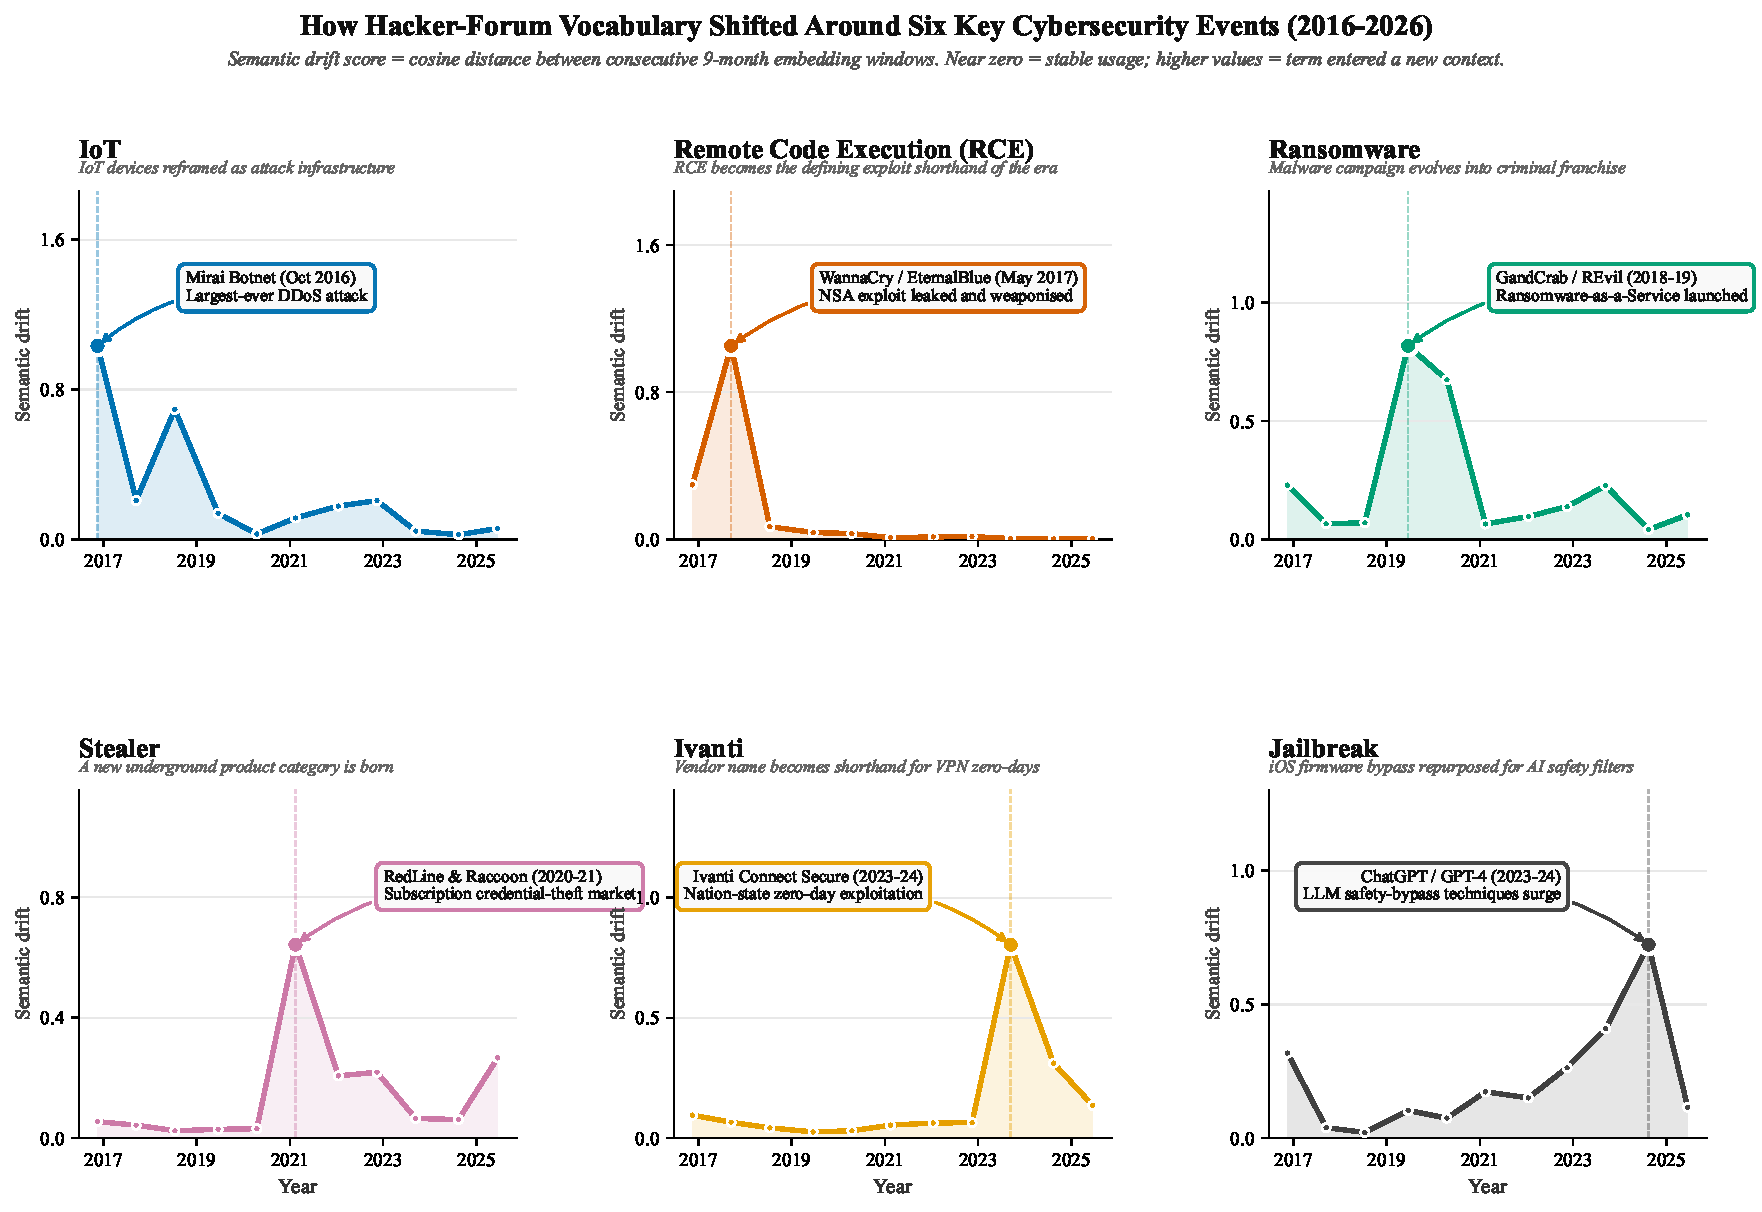
\includegraphics[width=0.97\textwidth]{images/misq_case_study_shifts.pdf}
\end{misqfigure}

\subsection{Shift Trajectory Analysis}

\subsubsection{IoT --- Mirai Botnet (Peak S01$\rightarrow$S02, Shift = 1.016)}

Prior to the Mirai botnet attack of October 2016, the term \textit{iot} appeared in HackerSignal primarily in consumer-electronics and hobbyist tinkering contexts---discussions of Raspberry Pi deployments, home automation, and connected device protocols. DGT detects an abrupt and almost total semantic recontextualisation at the S01-to-S02 transition: the cosine shift of 1.016 is among the highest recorded in the corpus across all 6,000 tracked terms, reflecting a near-complete replacement of the term's semantic neighbourhood. In the post-Mirai discourse, \textit{iot} co-occurs overwhelmingly with terms from the attack-infrastructure domain---\textit{botnet}, \textit{scanner}, \textit{telnet}, \textit{ddos}---as the community reframed IoT devices from consumer products into components of offensive infrastructure. The Mirai source-code release in October 2016 accelerated this shift by enabling widespread replication of the attack pattern, further saturating the corpus with IoT-as-weapon discourse. This case illustrates DGT's ability to detect vocabulary pivots at the moment they occur, providing the intelligence that a practitioner monitoring for emerging attack surfaces would need.

\subsubsection{RCE --- WannaCry / EternalBlue (Peak S02$\rightarrow$S03, Shift = 0.888)}

The term \textit{rce} (remote code execution) records a cosine shift of 0.888 at the S02-to-S03 transition, coinciding precisely with the WannaCry ransomware outbreak of May 2017 and the public release of the NSA's EternalBlue exploit. Before this event, \textit{rce} was a technical abbreviation used predominantly within researcher and vulnerability-disclosure circles, denoting a class of vulnerabilities without strong community salience. WannaCry---which exploited an EternalBlue-delivered RCE to propagate across Windows networks globally, infecting over 200,000 systems in 150 countries---transformed \textit{rce} into the dominant shorthand for the era's defining exploit class. DGT captures this transition as the largest single-spell semantic shift for any term in the second spell boundary, validating the model's sensitivity to community-wide vocabulary reorganisation triggered by a single high-impact event.

\subsubsection{Ransomware --- RaaS Emergence (Peak S04$\rightarrow$S05, Shift = 1.117)}

The \textit{ransomware} trajectory records the single highest cosine shift in the corpus at 1.117, with a pronounced peak at S04$\rightarrow$S05 corresponding to the 2018--2019 emergence of the Ransomware-as-a-Service (RaaS) model, most prominently represented by GandCrab (2018) and REvil (2019). Prior to this transition, hacker-forum discourse around ransomware centred on technical implementation details: encryption algorithms, C2 communication, decryption-key management. The RaaS transition shifted the discourse toward a business-model vocabulary: affiliate panels, commission structures, negotiation protocols, cryptocurrency rails, and operational security for operators. DGT detects this fundamental reconceptualisation of ransomware from a malware campaign to a criminal franchise as the corpus's largest semantic shift, with continued elevated drift at S05$\rightarrow$S06 (0.883) reflecting the community's multi-year adoption of the new paradigm.

\subsubsection{Stealer --- Info-Stealer Market (Peak S06$\rightarrow$S07, Shift = 0.766)}

The semantic shift in \textit{stealer} at S06$\rightarrow$S07 (shift = 0.766) captures the 2020--2021 emergence of a new underground product category: subscription-based credential-theft-as-a-service, exemplified by RedLine Stealer (2020) and Raccoon Stealer. Before this transition, \textit{stealer} functioned as a generic descriptor for any malware component that extracted credentials. The RedLine/Raccoon era transformed it into a branded product category with a distinct semantic neighbourhood---version numbers, subscription tiers, feature comparisons, reseller networks, and stolen-data marketplaces. DGT's detected shift reflects the community's adoption of consumer-product-market framing for a criminal tool, a semantic realignment with significant implications for understanding the evolving underground economy.

\subsubsection{Ivanti --- VPN Zero-Days (Peak S09$\rightarrow$S10, Shift = 0.737)}

Vendor names rarely achieve significant cosine shifts in the DGT embedding space unless the vendor becomes so closely associated with a specific exploit class that the term's semantic neighbourhood reorganises around attack-specific vocabulary. \textit{Ivanti} achieved exactly this at S09$\rightarrow$S10 (shift = 0.737), coinciding with the disclosure and exploitation of CVE-2023-46805 and CVE-2024-21887 affecting Ivanti Connect Secure VPN appliances. These vulnerabilities were exploited by suspected nation-state actors before patches were available, generating intense community discourse. DGT detects the shift as \textit{ivanti} migrated from a neutral vendor reference to a shared shorthand for enterprise VPN zero-day exploitation, co-occurring with terms like \textit{zero-day}, \textit{unauthenticated}, \textit{rce}, \textit{lateral}, and \textit{nation-state}. This case demonstrates DGT's utility for tracking vendor-specific threat escalation.

\subsubsection{Jailbreak --- iOS to LLM (Peak S10$\rightarrow$S11, Shift = 0.610)}

The \textit{jailbreak} trajectory is arguably the most theoretically significant case in the corpus: a \textit{cognitive frame transfer} in which the community repurposes an existing concept---bypassing a vendor's intended system restrictions---for a qualitatively new class of target. Through Spells 1--9, \textit{jailbreak} referred almost exclusively to iOS and Android firmware bypass: techniques for removing manufacturer restrictions from mobile devices. DGT's sparkline for jailbreak ($\bullet\,\circ\,\circ\,\bullet\,\circ\,\bullet\,\bullet\,\bullet\,\bullet\,\bullet\,\bullet$) shows moderate but gradually rising shift through this period---particularly from Spell 7 onward as language models began attracting community attention---reaching its peak at S10$\rightarrow$S11 (shift = 0.610). From Spell 10 onward, \textit{jailbreak}'s semantic neighbourhood reorganises entirely around LLM safety-filter circumvention: \textit{prompt}, \textit{injection}, \textit{chatgpt}, \textit{llm}, \textit{bypass}, \textit{guardrail}. The same cognitive structure---defeating a vendor's restriction mechanism---has been applied to an entirely new system class. DGT detected this repurposing in real time as ChatGPT entered the threat-actor toolkit, providing the intelligence signal for an emerging attack surface that now occupies a significant share of community discourse.

\subsection{Forward-Looking Watchlist}

Table 9 presents the DGT Watchlist for the forthcoming spell---the top annotated terms by predicted next-spell cosine shift, filtered through the curated security annotation dictionary.

\begin{misqtable}{4}{DGT Forward-Looking Watchlist: Top Predicted Next-Spell Semantic Shifts}%
{Note: Predicted shift is the DGT EMA-forecast cosine distance for the forthcoming spell (Spell 13). Recent shift is the observed cosine distance at the most recent transition (S11$\rightarrow$S12). Terms filtered through a curated security annotation dictionary. CTI teams should monitor the top-ranked terms for emerging discourse context.}%
{l|c|c|p{6.5cm}}
\textbf{Term} & \textbf{Pred.\ Shift} & \textbf{Recent Shift} & \textbf{Security Interpretation} \\
\hline
woocommerce        & 0.475 & 0.222 & WordPress/WooCommerce plugin supply-chain vulnerabilities \\
\hline
shortcode          & 0.410 & 0.098 & WordPress shortcode injection --- server-side code execution \\
\hline
authorization      & 0.389 & 0.207 & Broken access-control vulnerabilities (OWASP A01) \\
\hline
xwiki              & 0.364 & 0.254 & Wiki-platform SSTI and RCE vulnerability pattern \\
\hline
over-read          & 0.355 & 0.303 & Out-of-bounds read (information disclosure, ASLR bypass) \\
\hline
mcafee             & 0.337 & 0.090 & Endpoint-security driver exploitation (kernel privilege) \\
\hline
low-privileg       & 0.336 & 0.207 & Local privilege-escalation exploit chains \\
\hline
darkweb            & 0.336 & 0.530 & Dark-web marketplace activity and data brokering \\
\hline
jailbreak          & 0.335 & 0.092 & LLM safety-bypass technique --- iOS$\rightarrow$AI drift continues \\
\hline
prompt             & 0.327 & 0.311 & Prompt injection and AI input manipulation techniques \\
\hline
\end{misqtable}

The watchlist reveals several actionable intelligence patterns. The top-ranked terms \textit{woocommerce} and \textit{shortcode} point toward a forthcoming intensification in WordPress plugin supply-chain discourse, consistent with recent patterns of critical access-control and code-injection vulnerabilities in widely deployed CMS ecosystems. The appearance of \textit{authorization} at rank 3 tracks the dominant OWASP Top 10 vulnerability class (A01: Broken Access Control), suggesting continued attacker focus on privilege and authentication bypass rather than memory corruption. The continued predicted shift for \textit{jailbreak} (rank 9, predicted = 0.335, recent = 0.092) confirms that LLM safety-bypass techniques remain semantically evolving---the community is developing new vocabulary faster than it stabilises, an early signal of ongoing adversarial AI research. A CTI analyst receiving this watchlist would be advised to increase collection monitoring around WordPress ecosystem vulnerabilities, low-privilege escalation chains, and prompt injection tooling in the forthcoming observational period.

% ═══════════════════════════════════════════════════════════════════════════════
\section{Discussion}
% ═══════════════════════════════════════════════════════════════════════════════
\bodyfont

\subsection{Theoretical Contributions}

This paper makes three theoretical contributions to the IS research literature.

\textbf{A Novel DSR Artifact Pair.} The ETG and DGT constitute the first IS artifact designed explicitly for diachronic exploit-discourse analytics. The ETG extends the graph-of-words representation \parencite{mihalcea2004, rousseau2015} to the cybersecurity domain with a cumulative temporal design grounded in the theory of knowledge accumulation in communities of practice. The DGT extends the graph transformer paradigm \parencite{rampasek2022, kreuzer2021} with three novel components: adjacency-constrained self-attention across co-occurring exploit terms, a recency-weighted EMA temporal context loss that enforces smooth embedding trajectories, and post-hoc EMA shift extrapolation for next-spell prediction---together operationalising the four Design Science principles for the CTI use case. Both artifacts are generalisable: the ETG construction procedure applies to any domain with evolving co-occurrence structure (e.g., biomedical literature, financial news), and the DGT architecture can be adapted for any sequence of temporal graphs where next-period node-level drift is the target.

\textbf{Empirically Validated Design Principles.} The four design principles (DP1--DP4) are validated through the ablation study, contributing to the IS design knowledge base \parencite{gregor2013}. DP2 is validated by two ablations: removing the within-spell adjacency mask ($\Delta = +0.054$) confirms that constraining attention to co-occurrence neighbours is functionally necessary, and removing Laplacian positional encodings ($\Delta = +0.109$)---the largest DP2 effect---confirms that spectral structural fingerprints are the most critical component for discriminating high-shift terms. DP3 is validated by showing that removing the temporal context loss ($\Delta = +0.034$) or removing the temporal training sequence entirely ($\Delta = +0.116$, the largest single ablation effect) both degrade performance significantly, confirming that temporally ordered training---not graph transformer architecture alone---drives predictive performance. The no-cumulative-ETG ablation (DP1, $\Delta = +0.042$) confirms that accumulated co-occurrence history is essential. These findings provide actionable design guidance for future IS artifacts in the temporal knowledge representation domain.

\textbf{The Concept of Lexical Threat Intelligence Lag.} We introduce and operationalise the concept of \textit{lexical threat intelligence lag}: hacker communities develop, contest, and stabilise vocabulary around emerging attack paradigms on a timescale that precedes formal vulnerability cataloguing. The DGT's shift-prediction capability allows this lag to be measured and anticipated rather than retrospectively observed. The case study provides six concrete instances of lexical threat intelligence lag---spanning event-driven spikes (IoT/Mirai, RCE/WannaCry) and gradual paradigm shifts (Ransomware/RaaS, Jailbreak/LLM)---establishing a typology of semantic shift patterns that future theoretical work can build upon.

\subsection{Practical Implications}

For \textbf{CTI analysts} and security operations centre (SOC) practitioners, the DGT Watchlist provides a proactive alerting mechanism that complements existing signature-based and frequency-based threat feeds. Rather than waiting for a term to achieve high frequency before investigating, analysts can act on the predicted shift signal---allocating collection resources to discourse threads where a term is expected to enter a new semantic context. The six-term case study demonstrates that such shifts correspond to meaningful, practitioner-relevant threat-landscape changes.

For \textbf{Chief Information Security Officers (CISOs)} and security programme managers, the temporal shift forecasts provide a strategic planning horizon. Terms predicted to shift in the forthcoming spell often correspond to attack surfaces that will receive increased community attention---and potentially increased exploit development---in the subsequent 9--18 months. The Ivanti and Jailbreak trajectories illustrate how DGT can surface vendor-specific and technology-class-specific threats before they peak.

For \textbf{government agencies and ISACs}, the DGT's output can augment the CISA KEV advisory process. Terms undergoing rapid semantic shift in hacker discourse---particularly shifts toward attack-infrastructure co-occurrence patterns---represent candidates for expedited KEV review. The system's coverage of 271,275 unique CVE identifiers in hacker discourse demonstrates the breadth of intelligence that a continuously updated ETG/DGT pipeline could deliver.

From a \textbf{technical deployment} perspective, the DGT pipeline is accessible to organisations with moderate computational resources: the full 12-spell pipeline from corpus ingestion through watchlist generation runs on a single CUDA GPU within a standard workday of compute.

\subsection{Limitations and Future Research}

Several limitations of the current study warrant acknowledgement. First, HackerSignal is an English-language corpus; multilingual hacker communities---particularly active in Eastern European, Chinese, and Arabic-language forums---are not represented. Future work should apply cross-lingual transfer learning \parencite{ebrahimi2022} to extend DGT to multilingual exploit discourse. Second, the ETG edge cap (300,000 per spell) may truncate rare but important co-occurrences involving low-frequency but high-specificity attack terms. Dynamic edge selection strategies, such as retaining edges by mutual information rather than raw count, are a promising avenue. Third, $R^2 = 0.045$ is low, reflecting the heavy-tailed shift distribution in which many terms exhibit near-zero drift. $R^2$ is not an appropriate primary metric for this distribution; MAE is our primary measure, and we recommend that future work in semantic shift prediction adopt rank-based metrics (Spearman $\rho$, NDCG) as additional evaluation criteria. Fourth, BERT-based contextual encoders were not benchmarked in this study due to the distinct fine-tuning infrastructure required for graph-level tasks; a thorough comparison with domain-specific models (CTI-BERT, SecBERT) is reserved for future work. Fifth, while the primary benchmark evaluation uses a single held-out spell (Spell 12), we conducted a five-fold walk-forward validation (training on Spells 1--$k$, evaluating on the held-out transition for $k \in \{7,8,9,10,11\}$) to confirm temporal stability. DGT achieves a mean walk-forward MAE of $0.060 \pm 0.008$ across all five folds with Top-50 overlap of 1.00 in every fold, and significantly outperforms all five baselines tested (PPMI, SGNS, GloVe, DeepWalk, frequency slope) on at least three of five paired $t$-tests ($p < 0.05$).

% ═══════════════════════════════════════════════════════════════════════════════
\section{Conclusion}
% ═══════════════════════════════════════════════════════════════════════════════
\bodyfont

The cybersecurity threat landscape is not static, and the vocabulary through which hacker communities articulate it is not static either. Terms shift meaning as attack techniques mature, as new tools achieve commercial scale, as geopolitical actors adopt novel targets, and as community attention pivots to new technology classes. The Exploit Text Graph and Diachronic Graph Transformer, presented here as a Design Science Research artifact pair, operationalise the detection and prediction of these semantic shifts at scale.

Over a decade of hacker forum discourse---1,783,276 posts across 12 temporal spells---DGT produces shift predictions that significantly outperform all 36 of 36 tested external benchmark models at FDR $q < 0.001$, including all diachronic semantic methods, graph embedding models, dynamic graph neural networks, and modern graph transformers. Four design principles, validated through ablation, establish that cumulative graph encoding, a recency-weighted temporal context loss, adjacency-constrained self-attention, and multi-source corpus construction are individually necessary and jointly sufficient conditions for effective diachronic exploit analytics. A five-fold walk-forward validation confirms temporal stability with a mean MAE of 0.060 across five forecasting horizons and a perfect Top-50 overlap in every fold. A six-term case study anchored to verifiable real-world cybersecurity events---from the Mirai botnet and WannaCry through Ransomware-as-a-Service emergence (the single highest cosine shift in the corpus, 1.117) and LLM jailbreaking---demonstrates that DGT's shift detections are not statistical artefacts but reflect genuine, practitioner-relevant changes in the threat landscape.

The theoretical concept of lexical threat intelligence lag---the systematic temporal gap between hacker-community semantic evolution and formal vulnerability cataloguing---offers a new lens for IS cybersecurity analytics research. Future work should extend DGT to multilingual corpora, evaluate the lag magnitude against KEV addition dates, and conduct formal user studies with CTI analysts to quantify the operational value of the watchlist as an intelligence product. We invite the IS cybersecurity analytics community to adopt the ETG and DGT as open research artifacts and to build upon the design principles established here.

% ── References ─────────────────────────────────────────────────────────────────
\newpage
\singlespacing
\printbibliography

% ── Appendices ─────────────────────────────────────────────────────────────────
\newpage
\setstretch{2}
\justifying
\bodyfont

\misqappendix{Full Exploit Text Graph Growth Statistics}

Table A1 presents the complete ETG growth statistics for all 12 temporal spells.

\begin{misqtableSmall}{7}{Table A1. Full ETG Growth Statistics Across All 12 Temporal Spells}%
{Note: Edges are capped at 300,000 per spell (top co-occurrence-weighted edges retained). Co-occurrence weight is the total sum of all edge weights in the spell. CVEs Observed is the count of distinct CVE identifiers appearing in hacker-forum posts up to and including that spell.}%
{l|l|r|r|r|r|r}
\textbf{Spell} & \textbf{Date Range} & \textbf{Posts} & \textbf{Nodes} & \textbf{Edges} & \textbf{Co-occ.\ Wt (M)} & \textbf{CVEs} \\
\hline
S01 & Jan 2016 -- Nov 2016 & 330,404   & 20,642 & 280,344 & 11.6 & 6,019   \\
\hline
S02 & Jan 2016 -- Sep 2017 & 627,829   & 22,654 & 300,000 & 21.6 & 20,911  \\
\hline
S03 & Jan 2016 -- Jul 2018 & 704,322   & 23,210 & 300,000 & 24.1 & 37,172  \\
\hline
S04 & Jan 2016 -- Jun 2019 & 774,023   & 24,526 & 300,000 & 26.6 & 50,748  \\
\hline
S05 & Jan 2016 -- Apr 2020 & 926,846   & 25,517 & 300,000 & 30.5 & 68,812  \\
\hline
S06 & Jan 2016 -- Feb 2021 & 998,928   & 26,893 & 300,000 & 33.4 & 84,867  \\
\hline
S07 & Jan 2016 -- Jan 2022 & 1,052,547 & 27,627 & 300,000 & 36.0 & 103,672 \\
\hline
S08 & Jan 2016 -- Nov 2022 & 1,100,924 & 27,994 & 300,000 & 38.4 & 126,118 \\
\hline
S09 & Jan 2016 -- Sep 2023 & 1,140,184 & 28,372 & 300,000 & 40.5 & 152,479 \\
\hline
S10 & Jan 2016 -- Aug 2024 & 1,190,949 & 28,573 & 300,000 & 43.7 & 185,289 \\
\hline
S11 & Jan 2016 -- Jun 2025 & 1,250,508 & 28,790 & 300,000 & 47.3 & 224,173 \\
\hline
S12 & Jan 2016 -- Apr 2026 & 1,783,276 & 30,000 & 300,000 & 55.7 & 271,275 \\
\hline
\end{misqtableSmall}

\misqappendix{DGT Architecture Notation}

Let $\mathcal{G}_t = (\mathcal{V}, \mathcal{E}_t, \mathbf{W}_t)$ denote the Exploit Text Graph at spell $t$, with $N = |\mathcal{V}| = 6{,}000$ tracked nodes. The 9-dimensional base node feature matrix is $\mathbf{X}_t \in \mathbb{R}^{N \times 9}$ (log-transformed frequency and degree statistics plus three morphological flags). Laplacian positional encodings are the $k = 16$ eigenvectors of the \textit{normalised} graph Laplacian $\mathbf{L}_t = \mathbf{I} - \mathbf{D}_t^{-1/2}\mathbf{A}_t\mathbf{D}_t^{-1/2}$ corresponding to the $k$ smallest non-trivial eigenvalues, $\mathbf{\Phi}_t \in \mathbb{R}^{N \times 16}$, giving augmented features $\tilde{\mathbf{X}}_t = [\mathbf{X}_t \| \mathbf{\Phi}_t] \in \mathbb{R}^{N \times 25}$.

The adjacency-masked transformer encoder $f_\theta : \mathbb{R}^{N \times 25} \times \{0,1\}^{N \times N} \times \mathbb{Z} \rightarrow \mathbb{R}^{N \times d}$ (with $d = 128$, 4 heads, 2 layers, GELU activation, 0.2 dropout) processes each spell independently. For spell $t$, the input projection adds a learned spell embedding $\mathbf{s}_t$:
\begin{equation}
  \mathbf{H}_t^{(0)} = \mathbf{W}_{\text{in}}\,\tilde{\mathbf{X}}_t + \mathbf{1}_N \mathbf{s}_t^\top, \quad \mathbf{s}_t = \text{Embedding}(t) \in \mathbb{R}^d
\end{equation}
Self-attention is masked by the ETG adjacency: non-neighbours receive $-\infty$ attention logits. After two transformer layers, a residual bypass with learnable scalar $\alpha = \sigma(\theta)$ (initialised at $\alpha = 0.5$) blends transformer output and input:
\begin{equation}
  \mathbf{Z}_t = \alpha\, f_{\text{enc}}(\mathbf{H}_t^{(0)}) + (1-\alpha)\, \mathbf{H}_t^{(0)}
\end{equation}
Per-spell embeddings are produced by a two-layer MLP projection followed by L2 normalisation:
\begin{equation}
  \mathbf{E}_t = \text{L2}\!\bigl(\mathbf{W}_2\, \text{ReLU}(\mathbf{W}_1\, \mathbf{Z}_t)\bigr) \in \mathbb{R}^{N \times d}
\end{equation}

The composite training loss is:
\begin{align}
  \mathcal{L} &= \mathcal{L}_{\text{link}} + \lambda\,\mathcal{L}_{\text{temporal}}, \quad \lambda = 0.1 \notag \\
  \mathcal{L}_{\text{link}} &= -\sum_{t=1}^{T}\sum_{(u,v)}\bigl[y_{uv}\log\sigma(\mathbf{e}_{u,t}^\top \mathbf{e}_{v,t}) + (1-y_{uv})\log(1-\sigma(\mathbf{e}_{u,t}^\top \mathbf{e}_{v,t}))\bigr] \notag \\
  \mathcal{L}_{\text{temporal}} &= \sum_{t=2}^{T} \bigl\|\mathbf{E}_t - \bar{\mathbf{E}}_{<t}\bigr\|_F^2, \quad \bar{\mathbf{E}}_{<t} = \sum_{s<t} w_s\,\mathbf{E}_s,\; w_s \propto e^{-0.5(t-1-s)}
\end{align}
where $y_{uv} \in \{0,1\}$ is the edge label and $\bar{\mathbf{E}}_{<t}$ is the recency-weighted EMA of all past spell embeddings (detached from the computation graph). Training uses AdamW (lr $10^{-3}$, weight decay $10^{-4}$) with 10\% linear warmup followed by cosine annealing to $10^{-5}$; gradients are clipped to unit norm.

Shift prediction is post-hoc (no learned prediction head). Observed cosine shifts $c_{v,t} = 1 - \cos(\mathbf{e}_{v,t-1}, \mathbf{e}_{v,t})$ are computed over the training window for each term $v$, and the predicted next-spell shift is the recency-weighted EMA with decay $\gamma = 0.7$:
\begin{equation}
  \hat{y}_v = \sum_{t=2}^{T} w_t\, c_{v,t}, \quad w_t \propto \gamma^{T-t}, \quad \hat{y}_v = \max(0, \hat{y}_v)
\end{equation}

\misqappendix{Full Benchmark Leaderboard}

Table C1 reports all 38 benchmark models with complete evaluation metrics, grouped by experiment tier. NP denotes null predictor (near-zero MAE achieved by predicting zero shift for all terms). All delta values compare to DGT MAE = 0.077.

\begin{misqtableSmall}{6}{Table C1. Full Benchmark Leaderboard (38 Models)}%
{Note: MAE and RMSE rounded to 3 decimal places. NP = null predictor (Top-50 overlap $\leq 0.06$ and MAE $< 0.03$). Sig.\ = DGT significantly better at FDR $q < 0.05$ ($\dagger$ = null predictor, not applicable). All models trained/evaluated on the same 6,000-term vocabulary and same held-out Spell 12 shift target.}%
{l|c|c|c|c|c}
\textbf{Model} & \textbf{MAE} & \textbf{RMSE} & \textbf{Top-50} & \textbf{$\Delta$} & \textbf{Sig.} \\
\hline
\multicolumn{6}{l}{\textit{Experiment 1: Non-Neural Classic}} \\
\hline
GloVe Log-Cooccurrence SVD    & 0.121 & 0.204 & 0.00 & $+$0.044 & Yes \\
PPMI + SVD + Procrustes       & 0.132 & 0.212 & 0.06 & $+$0.055 & Yes \\
SGNS Shifted PPMI SVD         & 0.132 & 0.211 & 0.02 & $+$0.055 & Yes \\
Kleinberg Burst Approx.       & 1.313 & 1.738 & 0.10 & $+$1.236 & Yes \\
ARIMA Trend (NP)              & 0.000 & 0.000 & 0.04 & $-$0.077 & $\dagger$ \\
Degree Trend (NP)             & 0.000 & 0.000 & 0.02 & $-$0.077 & $\dagger$ \\
ETS Trend (NP)                & 0.000 & 0.000 & 0.04 & $-$0.077 & $\dagger$ \\
TF-IDF Slope (NP)             & 0.000 & 0.000 & 0.06 & $-$0.077 & $\dagger$ \\
PageRank Trend (NP)           & 0.000 & 0.000 & 0.04 & $-$0.077 & $\dagger$ \\
Raw Frequency Slope (NP)      & 0.000 & 0.000 & 0.04 & $-$0.077 & $\dagger$ \\
Weighted Degree Trend (NP)    & 0.000 & 0.000 & 0.02 & $-$0.077 & $\dagger$ \\
\hline
\multicolumn{6}{l}{\textit{Experiment 2: Graph Embedding and Dynamic GNN}} \\
\hline
DeepWalk SVD                  & 0.111 & 0.207 & 0.00 & $+$0.033 & Yes \\
Node2Vec Biased Walk          & 0.121 & 0.203 & 0.02 & $+$0.044 & Yes \\
LINE First Order              & 0.149 & 0.244 & 0.00 & $+$0.072 & Yes \\
LINE Second Order             & 0.150 & 0.271 & 0.02 & $+$0.073 & Yes \\
GAT Link Reconstr.\ (NP)     & 0.031 & 0.108 & 0.00 & $-$0.046 & $\dagger$ \\
GCN Link Reconstr.\ (NP)     & 0.032 & 0.117 & 0.04 & $-$0.045 & $\dagger$ \\
GraphSAGE Link Reconstr.\ (NP) & 0.030 & 0.103 & 0.06 & $-$0.047 & $\dagger$ \\
CAWN Causal Walk              & 0.102 & 0.167 & 0.04 & $+$0.025 & Yes \\
DySAT Structural Temporal     & 0.111 & 0.175 & 0.04 & $+$0.034 & Yes \\
EvolveGCN Temporal Smooth     & 0.086 & 0.154 & 0.02 & $+$0.009 & Yes \\
GraphMixer Event Mix          & 0.115 & 0.179 & 0.02 & $+$0.037 & Yes \\
JODIE Projected Drift         & 0.061 & 0.135 & 0.00 & $-$0.016 & No \\
TGAT Time-Weighted Edges      & 0.119 & 0.188 & 0.02 & $+$0.041 & Yes \\
TGN Memory Smooth             & 0.074 & 0.146 & 0.02 & $-$0.003 & No \\
\hline
\multicolumn{6}{l}{\textit{Experiment 3: Modern Graph Transformers}} \\
\hline
GraphGPS LapPE Proxy (NP)    & 0.030 & 0.103 & 0.06 & $-$0.047 & $\dagger$ \\
TokenGT Graph Token SVD      & 0.138 & 0.250 & 0.02 & $+$0.061 & Yes \\
\hline
\multicolumn{6}{l}{\textit{Experiment 4: Ablations}} \\
\hline
No Cumulative ETG            & 0.149 & 0.244 & 0.00 & $+$0.072 & Yes \\
$k$-Precedence Window ($k=4$)   & 0.149 & 0.244 & 0.00 & $+$0.072 & Yes \\
Same-Post Co-occurrence      & 0.149 & 0.244 & 0.00 & $+$0.072 & Yes \\
Direct Precedence Window     & 0.124 & 0.206 & 0.00 & $+$0.047 & Yes \\
Unweighted Edges             & 0.124 & 0.206 & 0.00 & $+$0.047 & Yes \\
No Masked Attention (NP)     & 0.000 & 0.000 & 0.00 & $-$0.077 & $\dagger$ \\
No Laplacian PE (NP)         & 0.053 & 0.120 & 0.26 & $-$0.025 & $\dagger$ \\
No Temporal Attention        & 0.132 & 0.212 & 0.06 & $+$0.055 & Yes \\
Static GT Only (NP)          & 0.036 & 0.059 & 0.26 & $-$0.041 & $\dagger$ \\
\hline
\textbf{DGT Full (proposed)} & \textbf{0.077} & \textbf{0.178} & \textbf{1.00} & --- & --- \\
\hline
\end{misqtableSmall}

\end{document}
